\documentclass[11pt]{article}
\title{\textbf{Aproximaci\'on a la soluci\'on de una ecuaci\'on diferencial ordinaria a trav\'es del m\'etodo de residuos ponderados}}
\author{Santiago Chialvo}
\date{Agosto 24, 2015}
\usepackage{amsmath}
\usepackage{graphicx}
\usepackage[latin1]{inputenc}
\usepackage[spanish]{babel}
\usepackage[T1]{fontenc}
\usepackage{color}
\usepackage{upquote}
%\usepackage{xcolor}
\usepackage{listings}
\usepackage{caption}
\usepackage{float}

\begin{document}

\lstset{language=Matlab,%
    %basicstyle=\color{red},
    breaklines=true,%
    morekeywords={matlab2tikz},
    keywordstyle=\color{blue},%
    morekeywords=[2]{1}, keywordstyle=[2]{\color{black}},
    identifierstyle=\color{black},%
    stringstyle=\color{green},
    commentstyle=\color{red},%
    showstringspaces=false,%without this there will be a symbol in the places where there is a space
    numbers=left,%
    numberstyle={\tiny \color{black}},% size of the numbers
    numbersep=9pt, % this defines how far the numbers are from the text
    emph=[1]{for,end,break},emphstyle=[1]\color{red}, %some words to emphasise
    %emph=[2]{word1,word2}, emphstyle=[2]{style},    
}

\maketitle


\section{Descripci\'on del problema}

Para este ejercicio se pide aproximar por el m\'etodo de los residuos ponderados la soluci\'on de la siguiente ecuaci\'on diferencial ordinaria:

\begin{equation}
\begin{aligned}
\frac{\delta^2\phi}{\delta x^2} + \phi = 0 \ \ \ \ \ \ 0 \leq x \leq 1 \\
\phi(x = 0) = 1 \\
\phi(x = 1) = 0
\end{aligned}
\end{equation}

\bigskip Para la cual la soluci\'on exacta est\'a dada por:

\begin{equation}
\phi = cos(x) - (cos(1)/sin(1))*sin(x)
\end{equation}

\bigskip Los m\'etodos para determinar las funciones de peso que se utilizar\'an ser\'an colocaci\'on puntual, colocaci\'on por subdominios y Galerkin. \bigskip

\section{Planteamiento y resoluci\'on del problema}

Para resolver este problema, comenzamos diciendo que cuando utilizemos Galerkin vamos a considerar aproximaciones elegidas de forma tal que no satisfagan todas las condiciones de contorno. Esto equivale a decir que nuestra $\psi = 0$. Es por ello que para elegir las funciones de prueba independientemente de las condiciones de contorno se utiliza una expansi\'on igual a:

\begin{equation}
\phi \approx \hat{\phi} = \sum_{m=1}^M a_m N_m
\end{equation}

\bigskip Esta aclaraci\'on vale para decir que ahora no solamente tendremos residuo en el interior del dominio, sino tambi\'en en el borde, definido por:

\begin{equation}
\begin{split}
R_\Omega = A(\hat{\phi}) = \mathcal{L}\hat{\phi} + p \\
R_\Gamma = B(\hat{\phi}) = \mathcal{M}\hat{\phi} + r
\end{split}
\end{equation}

\bigskip Como sabemos, el m\'etodo de los residuos ponderados consiste en escribir [1]:

\begin{equation}
\int_\Omega W_l R_\Omega d\Omega + \int_\Gamma \bar{W_l} R_\Gamma d\Gamma = 0
\end{equation}

\bigskip Con las funciones de peso elegidas arbitrariamente. Desarrollando un poco esta \'ultima ecuaci\'on:

\begin{equation}
\begin{split}
\int_\Omega W_l (\mathcal{L}\hat{\phi} + p) d\Omega + \int_\Gamma \bar{W_l} (\mathcal{M}\hat{\phi} + r) d\Gamma = 0 \\
\int_\Omega W_l (\mathcal{L}(\sum_{m=1}^M a_m N_m) + p) d\Omega + \int_\Gamma \bar{W_l} (\mathcal{M}(\sum_{m=1}^M a_m N_m) + r) d\Gamma = 0
\end{split}
\end{equation}

\bigskip Esta \'ultima expresi\'on tiene M inc\'ognitas, y aplicado para $ l = 1,2,...,M$ obtenemos un sistema del tipo:

\begin{equation}
\begin{split}
\textbf{Ka = f} \\
K_{lm} = \int_\Omega W_l \mathcal{L} N_m d\Omega + \int_\Gamma \bar{W_l} \mathcal{M} N_m d\Gamma \ \ \ \ \ \ 1 \leq l,m \leq M \\
f_l = - \int_\Omega W_l p d\Omega - \int_\Gamma \bar{W_l} r d\Gamma \ \ \ \ \ \ 1 \leq l \leq M \\
\end{split}
\end{equation}

\bigskip Desarrollando la ecuaci\'on 2.5 para nuestro problema espec\'ifico, notando que la integral en los extremos se reduce a la evaluaci\'on de los puntos extremos del dominio (por ser un problema 1D) llegamos a la siguiente expresi\'on:

\begin{equation}
\begin{split}
\int_0^1 W_l R_\Omega dx + \left[\bar{W_l} R_\Gamma \right]_{x=0} + \left[\bar{W_l} R_\Gamma \right]_{x=1} = 0 \\ 
\int_0^1 W_l (\frac{\delta^2\hat{\phi}}{\delta x^2} + \hat{\phi}) dx + \left[\bar{W_l} (\hat{\phi}-1) \right]_{x=0} + \left[\bar{W_l} \hat{\phi} \right]_{x=1} = 0 \\ 
\int_0^1 W_l (\frac{\delta^2\hat{\phi}}{\delta x^2} + \hat{\phi}) dx + \left[\bar{W_l} (\hat{\phi}) \right]_{x=0} + \left[\bar{W_l} * (-1) \right]_{x=0} +  \left[\hat{W_l} \hat{\phi} \right]_{x=1} = 0 \\ 
\int_0^1 W_l (\frac{\delta^2\hat{\phi}}{\delta x^2} + \hat{\phi}) dx + \left[\bar{W_l} (\hat{\phi}) \right]_{x=0} +  \left[\bar{W_l} (\hat{\phi}) \right]_{x=1} = - \left[\bar{W_l} * (-1) \right]_{x=0} \\ 
\end{split}
\end{equation}

\bigskip Las funciones de peso $W_l \ y \ \bar{W_l}$ ser\'an determinadas seg\'un el m\'etodo escogido. 

\bigskip Por otro lado, cuando utilizemos colocaci\'on puntual y colocaci\'on por subdominios como m\'etodos para las funciones de peso, haremos que las condiciones de borde se cumplan exactamente, por lo que nuestra $\psi$ dejar\'a de ser cero. Nuestra $\hat{\phi}$ quedar\'a de forma similar a la ecuaci\'on (3), s\'olo que con un t\'ermino adicional $\psi$ sumando. La ecuaci\'on general nos quedar\'a entonces de la siguiente forma:

\begin{equation}
\begin{split}
\int_0^1 W_l (\frac{\delta^2\hat{\phi}}{\delta x^2} + \hat{\phi}) dx = - \int_0^1 W_l \mathcal{L}\psi dx 
\end{split}
\end{equation}

\bigskip Para resolver nuestro problema, utilizaremos las funciones de prueba siguientes:

\begin{equation}
\mathcal{M}\phi = \phi \ \ \ \ r=-1 \ \ en \ x=0 \\
\end{equation}
\begin{equation}
\mathcal{M}\phi = \phi \ \ \ \ r=0 \ \ en \ x=1 \\
\end{equation}
\begin{equation}
N_m = x^{(m-1)} \ \ \ \ (Galerkin) \\
\end{equation}
\begin{equation}
N_m = sin(m*pi*x) \ \ \ \ (Puntual \ y \ Subdominios) \\
\end{equation}
\begin{equation}
\psi = 0 \ \ \ \ (Galerkin) \\
\end{equation}
\begin{equation}
\psi = 1-x \ \ \ \ (Puntual \ y \ Subdominios) \\
\end{equation}
\begin{equation}
\mathcal{L} = \frac{\delta^2}{\delta x^2} + 1\\
\end{equation}

\bigskip
\subsection{Colocaci\'on puntual}

En este m\'etodo se anula el residuo en un conjunto finito de puntos $x_l$, y la ecuaci\'on final nos quedar\'ia de la forma

\begin{equation}
\begin{split}
\frac{\delta^2\hat{\phi}(x(l))}{\delta x^2}+ \hat{\phi}(x(l)) = - \left[\psi \right]_{x=x(l)} \\ 
\end{split}
\end{equation}

\bigskip 
\subsection{Colocaci\'on por subdominios}

En este m\'etodo el error integrado sobre determinadas subregiones definidas previamente debe ser nulo. La ecuaci\'on final nos quedar\'ia de la forma:

\begin{equation}
\begin{split}
\int_{x(l)}^{x(l+1)} (\frac{\delta^2\hat{\phi}}{\delta x^2} + \hat{\phi}) dx = - \int_{x(l)}^{x(l+1)} \mathcal{L} \psi \ dx
\end{split}
\end{equation}

\bigskip 
\subsection{Galerkin}

Este es uno de los m\'etodos mas utilizados y consiste en elegir $W_l = N_l$. Para este problema en particular se utiliza $W_l = N_l$ y $\bar{W_l} = -N_l$ La ecuaci\'on final nos quedar\'ia de la forma:

\begin{equation}
\begin{split}
\int_0^1 N_l (\frac{\delta^2\hat{\phi}}{\delta x^2} + \hat{\phi}) dx - \left[\bar{N_l} (\hat{\phi}) \right]_{x=0} -  \left[\bar{N_l} (\hat{\phi}) \right]_{x=1} = \left[\bar{N_l} * (-1) \right]_{x=0} 
\end{split}
\end{equation}
\bigskip

\section{Resultados obtenidos}

Con un valor de M=4, se han obtenido los resultados favorables, los cuales se observan en la figuras 1,2 y 3. En la tabla 1 se observa el error cuadr\'atico medio para cada m\'etodo de las funciones de peso a medida que se aumenta el M, y se observa como converge a cero.

\begin{figure}
	\centering
		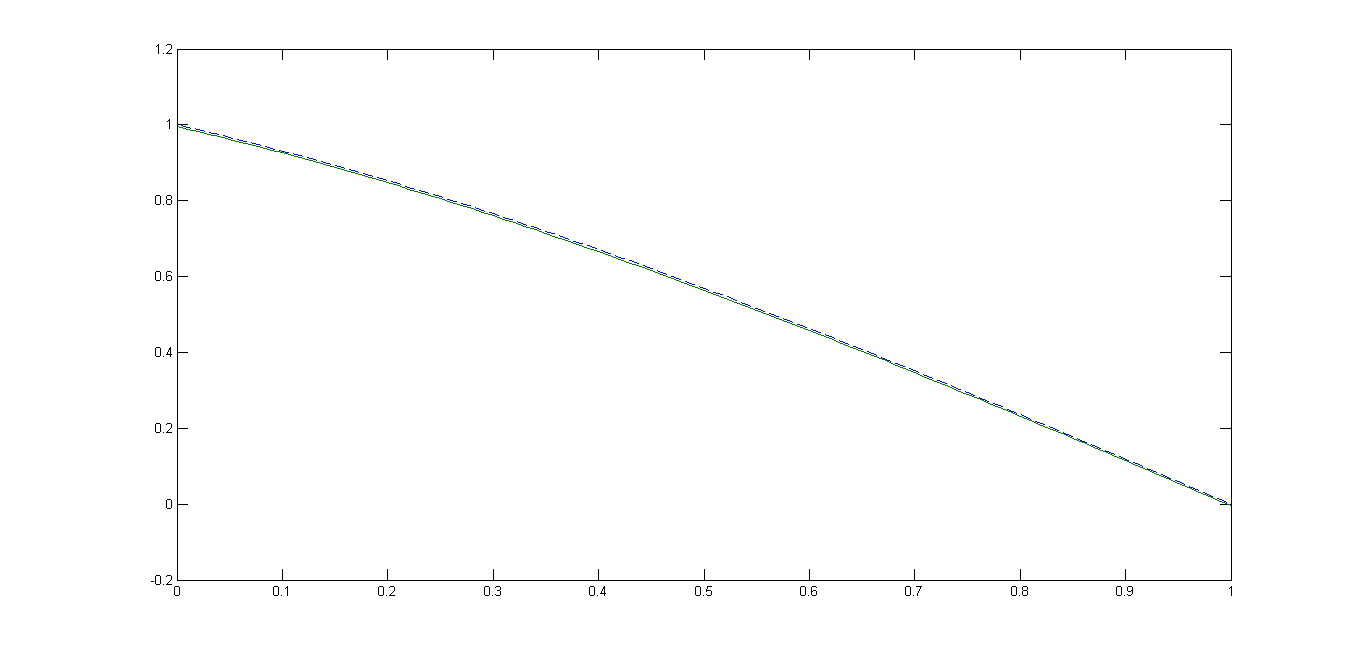
\includegraphics[width=1.0\textwidth]{Fig1.png}
	\caption{Aproximacion con M=4, utilizando Galerkin. Exacta (linea en rayas) y calculada (linea continua)}
	\label{fig:Fig1}
\end{figure}

\begin{figure}
	\centering
		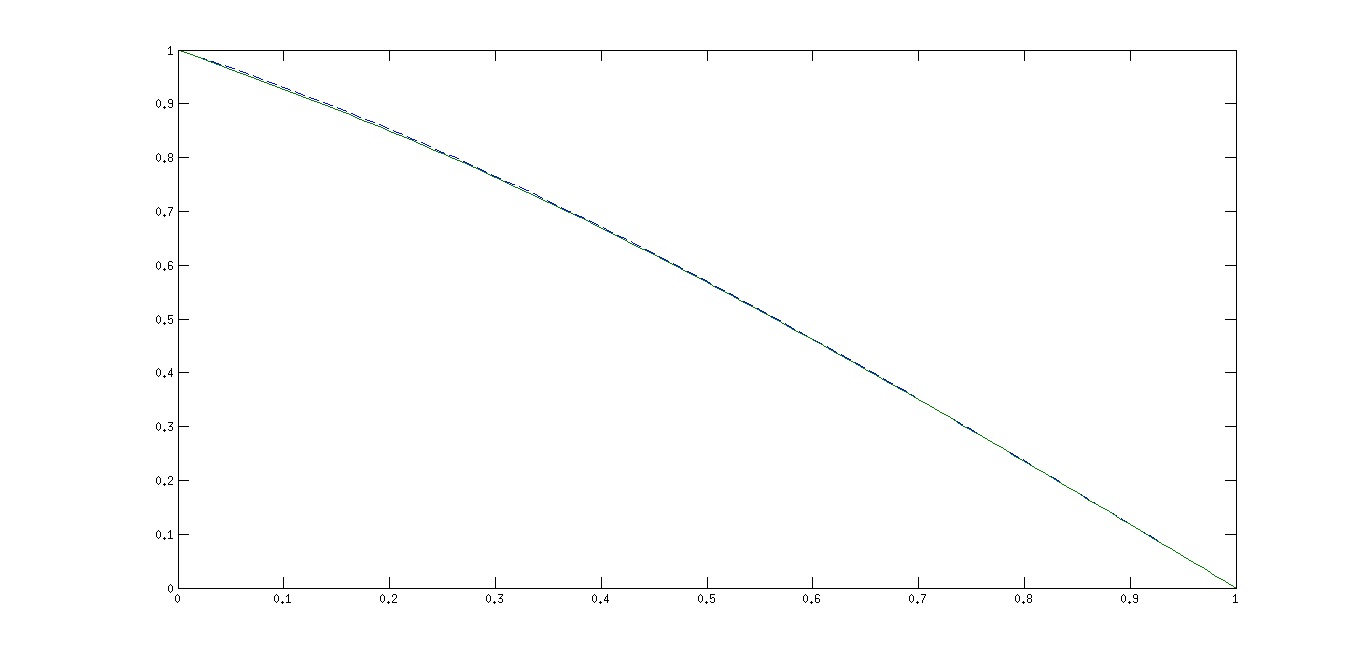
\includegraphics[width=1.0\textwidth]{Fig2.png}
	\caption{Aproximacion con M=4, utilizando colocaci\'on puntual. Exacta (linea en rayas) y calculada (linea continua)}
	\label{fig:Fig2}
\end{figure}

\begin{figure}
	\centering
		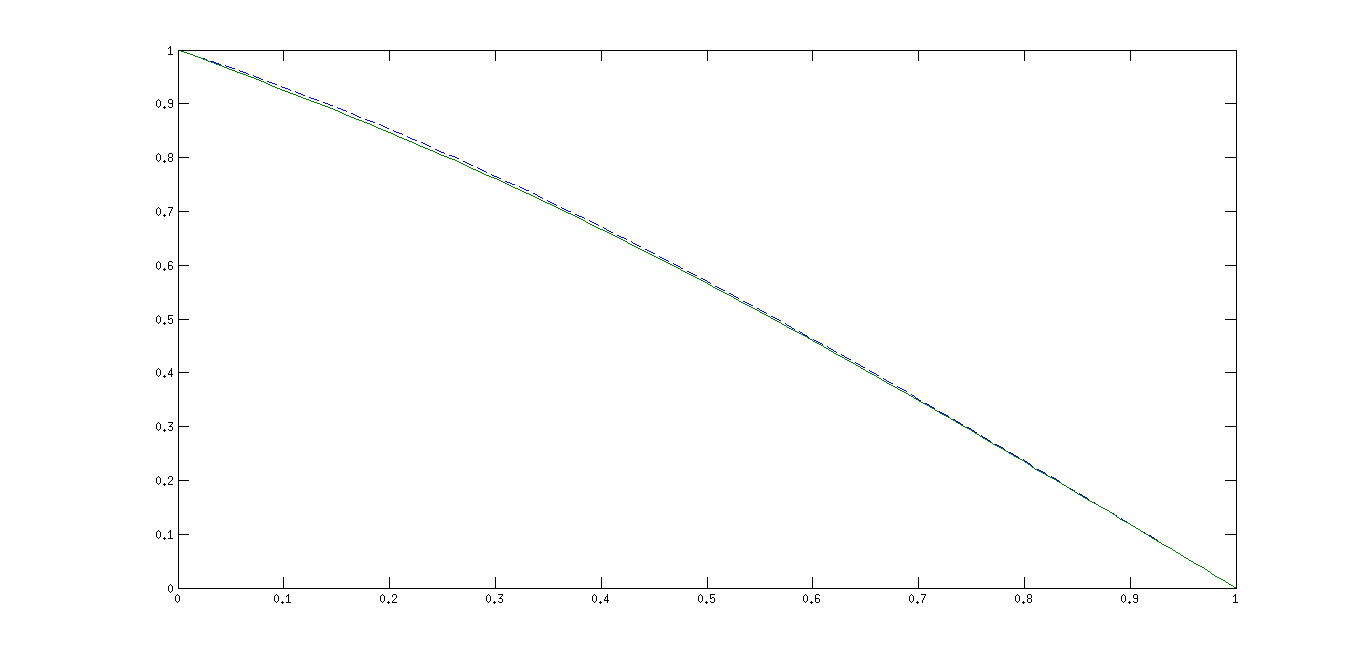
\includegraphics[width=1.0\textwidth]{Fig3.png}
	\caption{Aproximacion con M=4, utilizando colocaci\'on por subdominios. Exacta (linea en rayas) y calculada (linea continua)}
	\label{fig:Fig3}
\end{figure}

\begin{table}[h!]
\centering
\begin{tabular}{||c c c c||} 
 \hline
 M & Galerkin & C. Puntual & C. Subdominios \\ [0.5ex] 
 \hline\hline
 4 & 2.5400e-05 & 4.0937e-06 & 1.4355e-05 \\ 
 5 & 1.3123e-07 & 1.9848e-06 & 7.1294e-06 \\
 6 & 4.1307e-10 & 1.0756e-06 & 3.9281e-06 \\
 7 & 8.4604e-13 & 6.3242e-07 & 2.3378e-06 \\ [1ex] 
 \hline
\end{tabular}
\bigskip 
\caption{Error cuadr\'atico medio para cada m\'etodo de las funciones de peso a medida que aumenta el M}
\label{table:1}
\end{table}

\bigskip Observamos como, a pesar de que todos los m\'etodos dan resultados favorables, Galerkin tiene una convergencia del error a cero mucho mas r\'apida. Aunque quiz\'a no sea del todo 'correcto' comparar los m\'etodos dado que se utilizan diferentes $Nm$, la robustez de Galerkin se destaca sobre los dem\'as m\'etodos. 

\section{C\'odigo utilizado}

A continuaci\'on se presenta el c\'odigo utilizado para resolver el problema, escrito en el software Matlab.

\bigskip
\lstset{language=Matlab, breaklines=true, basicstyle=\footnotesize}
\begin{lstlisting}[frame=single]
%% Aproximacion a PDE por una funcion continua de prueba a traves del metodo de residuos ponderados

%% Utilizando funciones de peso
% 1-Galerkin
% 2-Colocacion Puntual
% 3-Subdominios

%Defino el dominio de la funcion

x=0:0.01:1;
lx=length(x);

%Numero de terminos usados para la aproximacion
M=7;

%Matriz K y vector F
K_1_s = sym(zeros(M,M));
K_2=zeros(M,M);
K_3_s = sym(zeros(M,M));
F_1=zeros(M,1);
F_2=zeros(M,1);
F_3=zeros(M,1);

%Se definen los puntos equiespaciados(Segun M)
delta_x=(max(x)-min(x))/(M+1); 
xc=zeros(M,1);

for i=1:M
  xc(i) = min(x)+i*delta_x;
end
xc(M+1)=max(x);

syms X N Deriv1_N Deriv2_N;
N=sym(zeros(1,M));

%Calculo los Nm para Galerkin
for i=1:M
    N(i)=X^(i-1);
end

%Lleno las matrices y el vector
for l=1:M,
 for m=1:M,
	 Deriv1_N = (1 - (m^2 * pi^2))*sin(m*pi*X); 
     Deriv2_N = (m-1)*(m-2)*X^(m-3) + X^(m-1);
     K_1_s(l,m) = int((Deriv2_N)*N(l),X,0,1) - (subs(N(m),X,0)*subs(N(l),X,0)) - (subs(N(m),X,1)*(subs(N(l),X,1))); 
	 K_2(l,m) = subs(Deriv1_N,X,xc(l));
     K_3_s(l,m) = int(Deriv1_N,X,xc(l),xc(l+1));
 end
 F_1(l)= subs(N(l),X,0)*-1;
 F_2(l)= -subs(1-X,X,x(l));
 F_3(l)= -int(1-X,X,xc(l),xc(l+1));
end

%Pasar de simbolo a numero 
K_1 = double(K_1_s);
K_3 = double(K_3_s);

% Computo la solucion
a_1 = K_1\F_1;
a_2 = K_2\F_2;
a_3 = K_3\F_3;

% Solucion exacta
phi_ex = (-cos(1)/sin(1))*sin(x) + cos(x); 
psi = 1-x;
phi_1=0;
phi_2=psi;
phi_3=psi;
% Solucion aproximada
for m=1:M,
  phi_1 = phi_1 + a_1(m)*(x.^(m-1));
  phi_2 = phi_2 + a_2(m)*sin(m*pi*x);
  phi_3 = phi_3 + a_3(m)*sin(m*pi*x);
end  


%Computo el error cuadratico medio
Err_1=0;
Err_2=0;
Err_3=0;
for i=1:length(x)
    Err_1=Err_1+(phi_ex(i)-phi_1(i))^2;
    Err_2=Err_2+(phi_ex(i)-phi_2(i))^2;
    Err_3=Err_3+(phi_ex(i)-phi_3(i))^2;
end

L = length(phi_ex);
Err_1=Err_1/L;
Err_2=Err_2/L;
Err_3=Err_3/L;

% Ploteo resultados
plot(x,phi_ex,'--',x,phi_3);
\end{lstlisting}
\bigskip

\newpage

\begin{thebibliography}{9}                                                                                                %
\bibitem {Nigro}Nigro, Norberto, Storti, Mario. \textit{M\'etodos Num\'ericos en Fen\'omenos de Transporte}, Centro Internacional de M\'etodos Computacionales en Ingenier\'ia, 2011.
\end{thebibliography}
\end{document}
